\documentclass[10pt,a4paper,spanish] {article}
\usepackage[spanish]{babel}
\usepackage[T1]{fontenc}
\usepackage[utf8]{inputenc}
\usepackage{graphicx}
\usepackage{tikz}
\usepackage{etex}


\begin{document}
\title{Nucleotide String Library}
\author{Juan José Delgado Quesada B42250\\José Ariel  Fallas Pizarro B42481\\David Martínez García B34019}

\maketitle

\section{Justificación}

Los nucleótidos son la base de nuestros genes. Estos se unen de manera única y específica para crear cada uno de los genes. Estos son únicos y se componen unicamente de 4 tipos de nucleótidos (Adenina, Guanina, Citosina, Timina). 
Una pequeña modificación en el código genético puede significarse una mutación, la cual podría terminar generando una especie completamente distinta a la originaria. 
Y el ADN de un organismo se compone de millones de millones de genes y comparar dos de ellos podría tomarse semanas e inclusive meses si se hace manualmente. Es por esto que automatizar este proceso es necesario, ya que si queremos descubrir una nueva especie o averiguar con cual especie de bacteria estamos tratando por ejemplo, podemos tomar una muestra de esta y compararla con una base de datos ya existente y hacerlo en cuestión de minutos.

\section{Objetivos General}

\begin{itemize}
\item Implementar una librer\'ia en C++ que facilite el trabajo y procesamiento de secuencias de bases nitrogenadas y a su vez permita trabajar con bases de datos de cadenas de bases nitrogenadas \textbf{(BLAST)}.
\end{itemize}

\subsection{Objetivos Específicos}
\begin{itemize}
\item Diseñar y estructurar las clases necesarias, que conformaran la Libreria para el manejo de bases nitrogenadas, con sus respectivas funciones.
\item Desarrollar una aplicación que permita poner en práctica las funciones y clases perteneciente a la libreria para el manejo de bases nitrogenadas.
\item Poner en práctica los conocimientos vistos en el curso de Estructuras Abstractas de Datos y Algoritmos para Ingeniería como lo son: el uso de Templates y el análisis de la efectividad.
\end{itemize}

\section{Desarrollo}
Para la realización de este proyecto se implementaron 3 clases fundamentales, las cuales tenian distintos propósitos 


\subsection{NucleoString}
	Esta clase tenía como objetivo hacer las operaciones con las cadenas de nucleótidos, tales como insertar, comparar, cortar, entre otras. 
	Con ello se pretende sistematizar y agilizar el proceso de busqueda de genes. La idea de esta clase es poder manejar cadenas de aminoácidos a nuestro gusto y de manera rápida.
	
\subsection{Management}
	El objetivo de esta clase era lograr comunicarse con la base de datos de internet de blast, para ello fue necesario bajar algunas de las librerias de blast ya existentes e implementarle algunas funciones nuevas.Para ello se necesitó descargar la librerías de blast y entender su funcionamiento. Sin esta clase sería imposible que la librería fuese útil, pues no tendría una base de datos con que compararse. Estas librerías de blast fueron escogidas pensando en que es la mayor base de datos de genes del mundo, por lo que tendría un mayor alcance
	
\subsection{Helix}
	Con esta clase se pretende relacionar cadenas de aminocácidos tal y como el ADN, el cual es una doble hélice. De esta forma se podría obtener una cadena y la complementaria de esta, pues ambas están enlazadas. 

\section{Análisis de eficiencia}

%\begin{center}
\begin{tabular}{|l|c|r|}
\hline
código & veces & operaciones\\
\hline
while(nucleo1.find(subconjunto)$<$npos)\ & n*n & c*n*n \\
i++ & 1 & j*n/2 \\
subconjunto.append(nucleo2.substr(n1+i)) & n(n/2) & m*n*(n/2)\\
subconjunto.push\_back(nucleo2.substr(n1-i));& n*n/2 & k*n*(n/2)\\
int aciertos = subconjunto.size(); & c & 1 \\
int totales  = nucleo1.size(); & 1 & \\
float porcentaje = aciertos/totales;  & 1 & 1 \\
return & const & 1\\
\hline
\end{tabular}
%\end{center}
\\
\newline
Resultado para el mejor caso se obtiene: \\

\begin{equation}
\label{eq:best}
c*n
\end{equation}


Resultado para el peor caso se tiene:\\

\begin{equation}
\label{eq:worst}
jn + \frac{m+k+2c}{2}*n^2
\end{equation}

Desarrollando la expresion anteriores y se obtiene la ecuación de T(n)

\begin{equation}
\label{eq:T(n)}
T(n)=\frac{a}{2}n^2 + dn 
\end{equation}

\section{Diagrama de Flujo}
\begin{figure}[h]
\centering
 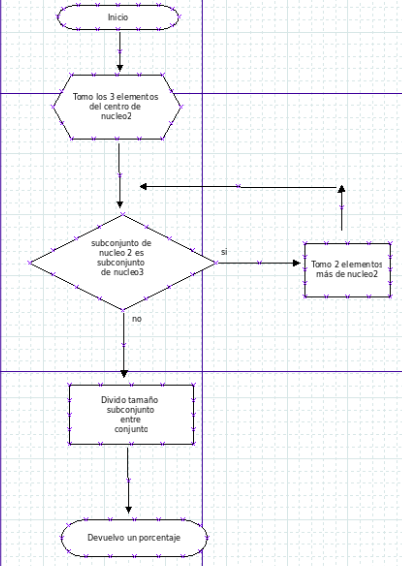
\includegraphics[width=3.0 in]{diagrama.png}
 \caption{Diagrama de flujo para compare}
 \label{flujo}

\end{figure}

\end{document}